\documentclass[11pt]{jarticle}
\usepackage[a4paper, margin=20mm]{geometry}
\usepackage{wrapfig}
\usepackage{jtygm}
\usepackage{listings}
\usepackage[usenames, dvipsnames]{color}
\usepackage[dvipdfmx]{graphicx}
\usepackage{keystroke}
\usepackage{menukeys}

\newcommand\gamename{サムライジョッキー}

\title{{\gamename}ゲームルール (暫定版)}
\author{情報処理学会プログラミングコンテスト委員会}
\date{2017/09/16}

\begin{document}
\maketitle

\begin{abstract}
  SamurAI Coding 2017--2018 に用いるゲームのルール案を述べる.
  このルール案は暫定版であり, 詳細については今後の改訂の可能性がある.
\end{abstract}

\section{ゲームの概要}
AIの制御するふたりのプレイヤがスタート位置から開始し, 障害物が設置され
たレースコース上でステップごとに位置を変えながら, ゴールに早く到達する
ことを競うゲームである.

1ゲームは, 同じレースコースを用い両プレイヤのスタート位置を交換した2レー
スからなる. 両レースのゴールタイムの合計が短い方がゲームの勝者である.
合計タイムが同一である場合は, そのゲームは引き分けである.

\begin{wrapfigure}{r}{0.38\columnwidth}
  \vspace{-2cm}
  \centering
  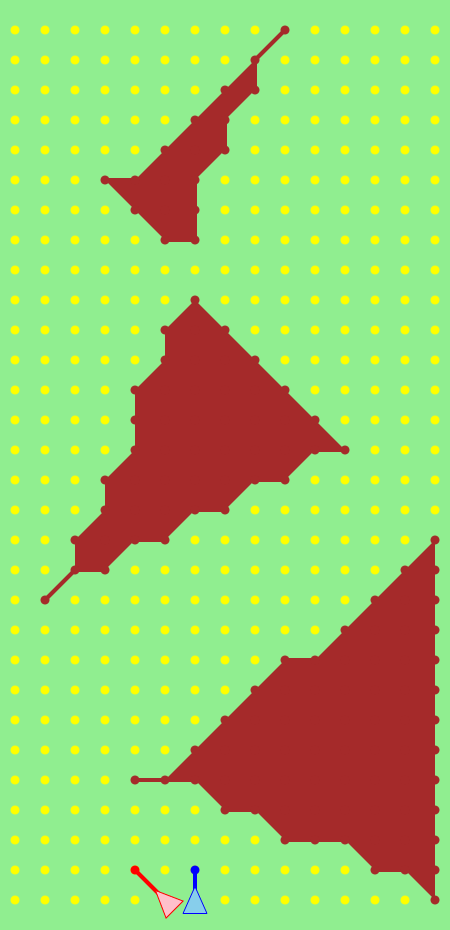
\includegraphics[width=0.35\columnwidth, natwidth=450, natheight=930]{racecourse.png}
  \caption{レースコースの例}
  \label{fig:course}
\end{wrapfigure}

\section{レースコース}
レースコースは2次元格子状であり, ゲーム毎に大きさや障害物の位置が異なる.
以下ではレースコースの幅を$w$, コース長を$l$とし,
各格子点の位置の座標を $(x,y)$ ($0\le x < w, 0\le y$) とする.

コース上の格子点の一部は{\bf 障害点}である.  障害点あるいは縦横斜めに
隣接するふたつの障害点を結んだ線分を{\bf 障害物}と呼ぶ. 障害物は固定さ
れており, レース中に動くことはない.  障害物を飛び越すことはできないの
で, 障害物に囲まれた領域に入ることはできない.

プレイヤを制御するAIプログラム (以下単に{\bf AI}と呼ぶ) に与えられる障
害物の情報は, プレイヤの視界の範囲内のもの, すなわちプレイヤの位置の前
後一定範囲の$y$座標にあるものについてのみである. 加減速は限定された範
囲でしかできないので, 速度を上げ過ぎると障害物を避けられなくなる可能性
がある.

図\ref{fig:course}にレースコースの例を示す. 茶色の小円は障害点, 線分や
塗りつぶした領域は障害物およびそれらに囲まれた領域である.

レース中, 両プレイヤはいずれかの相異なる格子点にある.  レース開始時の
両プレイヤの位置の$x$座標は異なり, $y$座標は$0$である.  両プレイヤはス
テップごとに位置を変えて行き, コース長$l$以上の$y$座標の地点に達したら
ゴールしたことになる.

コースには行き止まりがないものとする. コース内のどの格子点からも, 十分
小さい速度で移動すれば, 一度も$y$座標を減らすことなく障害物やコース端
にぶつからずに$y$座標がより大きい点に移動できる.

\section{レースの進行}
各レースでは, ステップごとにAIにレースの状況についての情報を与え, それ
に対するAIからの応答である加減速指示に従ってレースの状況を更新すること
を繰り返す.  レース中に両プレイヤが同時に同じ位置を占めることはない.

ステップは0から1ずつ進み, 両プレイヤ共にゴールすればレースは終了である.
ただし, 制限ステップ数に達してもゴールしないプレイヤがある場合, その時
点でレースは終了し, ゴールに達していないプレイヤのゴールタイムは制限ス
テップ数の2倍とする.

\subsection{考慮時間}
AIが1レースで使える{\bf 考慮時間}の合計には, 制限を設ける. 考慮時間は
ゲーム管理プログラムがプレイヤに情報を送信し終わってから, プレイヤから
の応答を受信し終わるまでの実時間である.  考慮時間の合計が制限値を超え
たプレイヤはそのレースを含むゲームを失う.
\footnote{考慮時間の制限値は未定だが, 数十秒程度となるだろう.}

\subsection{プレイヤの状態と加減速指示}
プレイヤは各ステップの開始時において{\bf 位置} $(x, y)$ と{\bf 速度}
$(v_x, v_y)$ を持つ.

AIはステップごとに速度を変更する{\bf 加速度} $(a_x, a_y)$を指定する.
$a_x, a_y$は各々$-1, 0, 1$のいずれかである.

後述するコースアウトや衝突によって動けない場合を除き, 次ステップのプレ
イヤの位置の座標は $(x+v_x+a_x, y+v_y+a_y)$ となる. この位置を以下では
次ステップにおける{\bf 予定位置}と呼ぶ. また, 次ステップにおけるプレイ
ヤの速度はコースアウトや衝突の有無に関わらず $(v_x+a_x, v_y+a_y)$ とな
る.

\begin{wrapfigure}{R}{0.28\columnwidth}
  \vspace{-1cm}
  \centering
  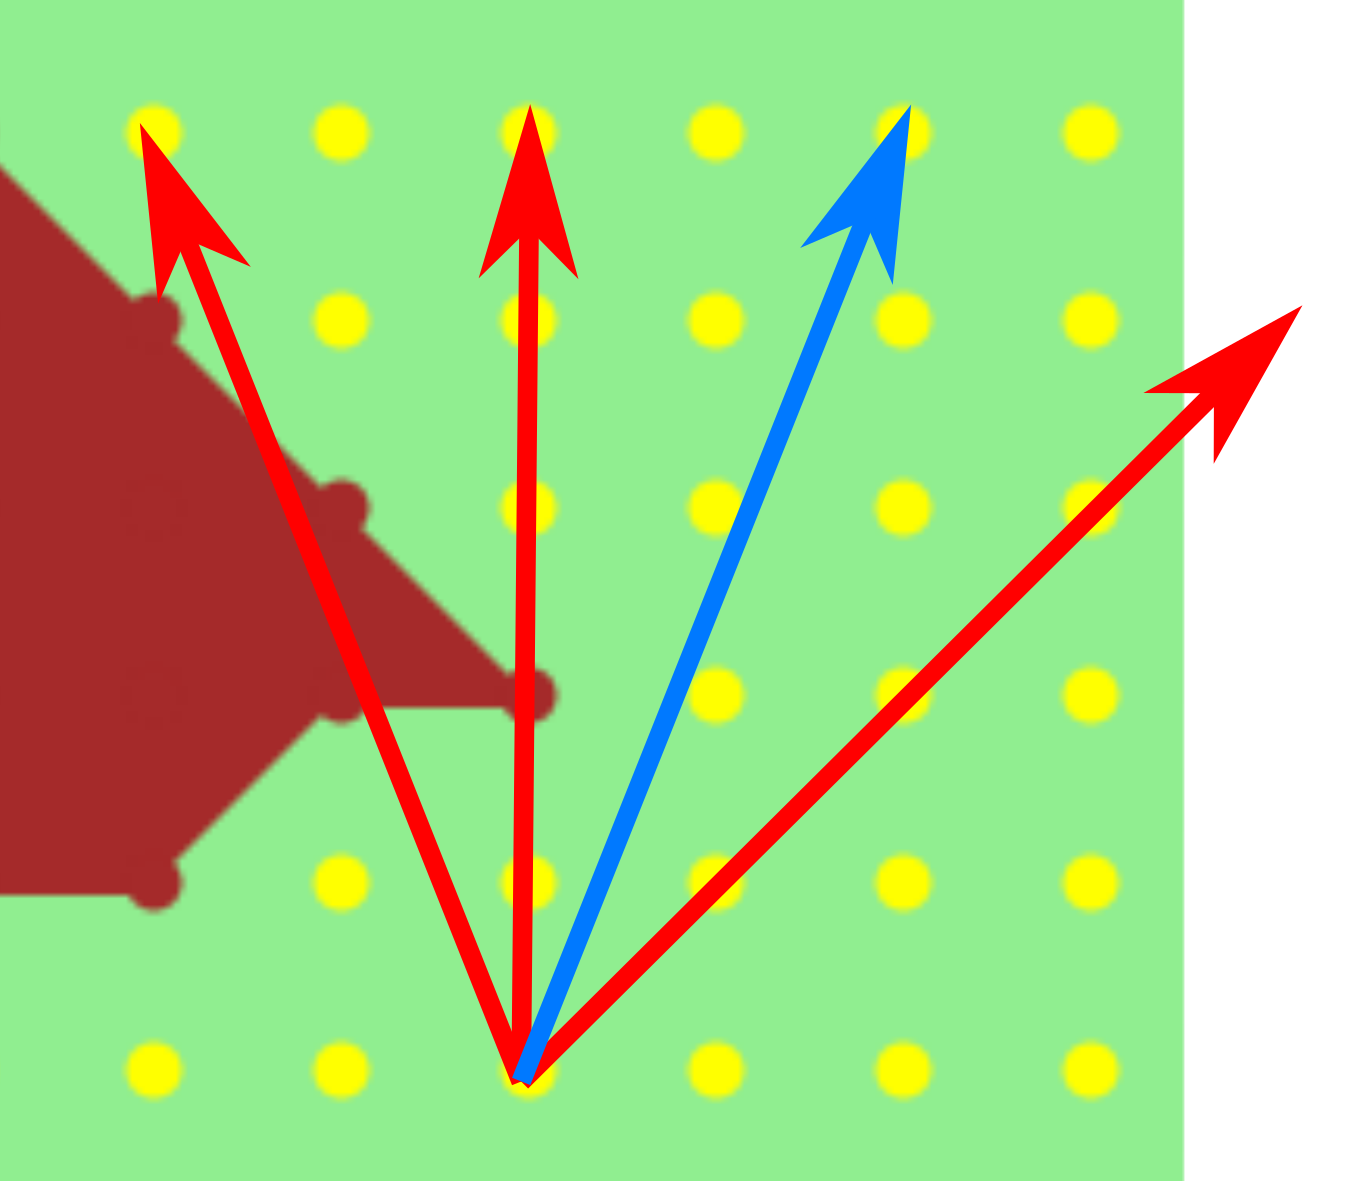
\includegraphics[width=0.26\columnwidth, natwidth=1358, natheight=1181]{courseout.png}
  \caption{コースアウト}
  \label{fig:courseout}
  赤い動線はコースアウト
  \vspace{-1cm}
\end{wrapfigure}

\subsection{動線とコースアウト}

プレイヤの位置と次ステップにおける予定位置を両端とする線分を, このプレ
イヤの当該ステップでの{\bf 動線}と呼ぶ.

以下の場合, 当該プレイヤは{\bf コースアウト}を生じているという.
\begin{itemize}
\item
  予定位置がコース外に出る, すなわち予定位置の座標$(x,y)$が$0 \le x <
  w$ かつ $0 \le y$ を満たさない場合
\item
  動線が障害物と交差あるいは接触する場合
\end{itemize}
コースアウトしたプレイヤの次ステップでの位置は元のままになる.  速度に
ついてはコースアウトしなかった場合と同じ加速度が適用される.

\begin{wrapfigure}{R}{0.32\columnwidth}
  \centering
  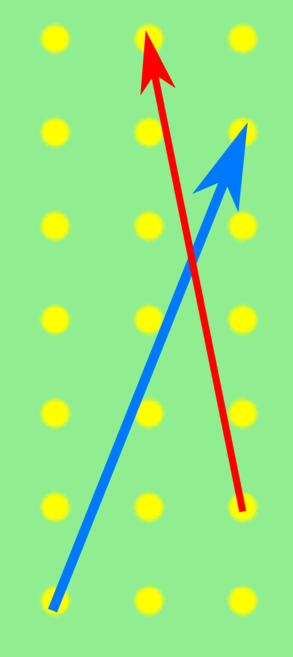
\includegraphics[scale=0.2, natwidth=293, natheight=657]{collision.png}
  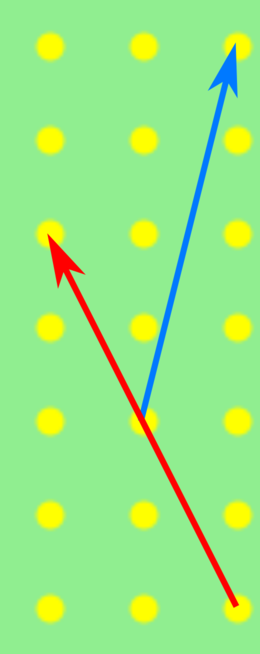
\includegraphics[scale=0.183, natwidth=288, natheight=657]{cropped.png}
  \caption{衝突}
  \label{fig:collision}
  いずれも青い動線のプレイヤが優先権を持つ
  \vspace{-1.5cm}
\end{wrapfigure}

\subsection{衝突と優先権}
コースアウトがない場合に, 両プレイヤの動線が交差あるいは接触する場合,
{\bf 衝突}が生じたという.

衝突が生じた場合は, {\bf 優先権}を持つプレイヤの次ステップの位置は予定
位置に, 優先権のないプレイヤの位置は元のままになる.  いずれのプレイヤ
についても, 次ステップの速度は衝突しなかった場合と同じ$(v_x+a_x,
v_y+a_y)$となる.

優先権を持つのは, 位置の$y$座標がより小さいプレイヤである.  $y$座標が
同一である場合, 位置の$x$座標がより小さいプレイヤが優先権を持つ. ただ
し, 動線が相手プレイヤの動作前の位置に達するか通過する場合は, 優先権
が相手プレイヤに移る.

両プレイヤとも互いに相手の位置に達するか通過するような動線を持つ場合は,
両者とも優先権を失い, 次のステップでの位置は元のままとなる.

\subsection{ゴールタイム}
プレイヤがステップ$s$で座標$(x, y)$の位置にあり, 次ステップで位置$(x',
y')$に達し, $y'\ge l$ ($l$ はコース長) であるとき, そのプレイヤはゴー
ルしたものとされる.  このときゴールタイムは$s + (l-y)/(y'-y)$で与えられる.

コースアウトしたプレイヤ, あるいは衝突を起こし優先権を持たないプレイヤ
は, たとえ予定位置の$y$座標がコース長以上であっても, 次ステップの位置
は元の位置のままとなるので, そのステップではゴールしない.

\section{AIの動作}
AIは初期化時にレース全体に関する情報を入力し, 初期化終了を示す応答を出
力する. ステップごとにはレース状況の情報を入力し, 応答として加速度指示
を出力する.

入力はひとつ以上の空白あるいは改行で区切った10進整数の並びである.
負の数にはマイナス符号を前置する.
初期化時の入力およびステップごとの入力の最後は必ず改行を置く.

AIの応答出力も空白あるいは改行で区切った10進整数の並びで, 負の数にはマ
イナス符号を前置する.  {\bf 出力の最後には必ず改行を置く.}

\subsection{初期化時の入力}
初期化時のAIの入力は以下の項目がこの順に並ぶものである.
\begin{description}
\item[考慮時間$t_{given}$] このレースで使える考慮時間をマイクロ秒単位の整数値として.
\item[制限ステップ数$s_{max}$] ゴールまでのステップ数の上限を整数値として.
\item[コースサイズ] コースの幅$w$および長さ$l$を, ふたつの整数値として.
\item[視界$d$] 視界に入る$y$座標の範囲を整数値$d$として.
  位置$(x,y)$にあるプレイヤを制御するAIをに与えられる相手プレイヤや障害点の情報は, 
  $y$座標が$y-d$から$y+d$の範囲 (両端を含む) にあるもののみが与えられる.
\end{description}

\makeatletter
\def\lst@visiblespace{$\color{Gray}{}_{
  \mbox{\kern.06em\vrule \@height.3ex}%
  \vbox{\hrule \@width.3em}%
  \hbox{\vrule \@height.3ex}}$}
\makeatother

\lstset{
  basicstyle=\ttfamily,
  frame = single,
  showspaces = true,
  escapeinside={<@}{@>},
  mathescape
}

\subsection{入力形式}
\begin{lstlisting}
$t_{given}$<@\tiny{\keys{\return}}@>
$s_{max}$<@\tiny{\keys{\return}}@>
$w$ $l$<@\tiny{\keys{\return}}@>
$d$<@\tiny{\keys{\return}}@>
\end{lstlisting}

\subsection{初期化時の出力}
AIは初期化が終了したことを整数$0$ひとつで伝える.

\begin{lstlisting}
0<@\tiny{\keys{\return}}@>
\end{lstlisting}

\subsection{ステップごとの入力情報}
ステップごとのAIの入力は以下の項目がこの順に並ぶものである.
\begin{description}
\item[ステップ$s$] 当該のステップの値を整数ひとつで与える.
\item[残り考慮時間$t_{left}$] このレースで使える考慮時間の残りをマイクロ秒単位の整数値として.
\item[自プレイヤの状態] 当該のAIが制御するプレイヤの位置の$x$座標と$y$座標, 速度の$x$成分$v_x$と$y$成分$v_y$の4整数.
\item[相手プレイヤの状態] 相手プレイヤの位置の$x$座標$ex$と$y$座標$ey$, 速度の$x$成分$ev_x$と$y$成分$ev_y$の4整数.
  ただし, 相手プレイヤの位置が視界の外であれば, $y$座標は$-1$, 他は$0$になる.
\item[障害点] 視界内の各格子点が障害点であるか否かの情報で,
  $(2\times d+1)\times w$個の整数からなる. 視界内の$y-d$から$y+d$までの各$y$
  座標に対して$w$個の整数$o_{0,y}, o_{1,y}, \ldots, o_{w-1,y}$が, $y$
  座標の順に与えられる.  $o_{x,y}$が$1$ならば格子点$(x,y)$は障害点であ
  り, $0$ならばそうではない.  ただし, $y<0$であるコース外の格子点につ
  いては$1$が与えられる.
\end{description}

\subsection{入力形式}
\begin{lstlisting}
$s$<@\tiny{\keys{\return}}@>
$t_{left}$<@\tiny{\keys{\return}}@>
$x$ $y$ $v_x$ $v_y$<@\tiny{\keys{\return}}@>
$x_e$ $x_e$ $v_{x_e}$ $v_{y_e}$<@\tiny{\keys{\return}}@>
$o_{0,y-d}$ $o_{1,y-d}$ ... $o_{w-1,y-d}$<@\tiny{\keys{\return}}@>
$o_{0,y-d+1}$ $o_{1,y-d+1}$ ... $o_{w-1,y-d+1}$<@\tiny{\keys{\return}}@>
...
$o_{0,y+d}$ $o_{1,y+d}$ ... $o_{w-1,y+d}$<@\tiny{\keys{\return}}@>
\end{lstlisting}

\subsection{ステップごとの出力}
AIは当該ステップの加速度$(a_x,a_y)$をふたつの整数で指定する.

\begin{lstlisting}
$a_x$ $a_y$<@\tiny{\keys{\return}}@>
\end{lstlisting}

\subsection{情報の記憶}
ゲーム管理システムは, 各ステップについて出力を終了したAIの動作を一時停
止し, 次ステップの情報を与える際に動作を再開させる.  このため, ステッ
プの間に計算を進めることはできないが, 変数値などの実行コンテキストは1
レースの間保持し続けることができる.

AIはファイル出力やネットワークアクセスができない環境で動作し, ゲーム管
理システムはレース毎にAIを初期状態から立ち上げ直す. このため, AIは複数
のレース間で情報を受け渡すことができない.

\begin{flushright}
以上
\end{flushright}

\end{document}
